\documentclass{standalone}

\usepackage{TikzStyle}
\usepackage{mystyle}

\begin{document}
    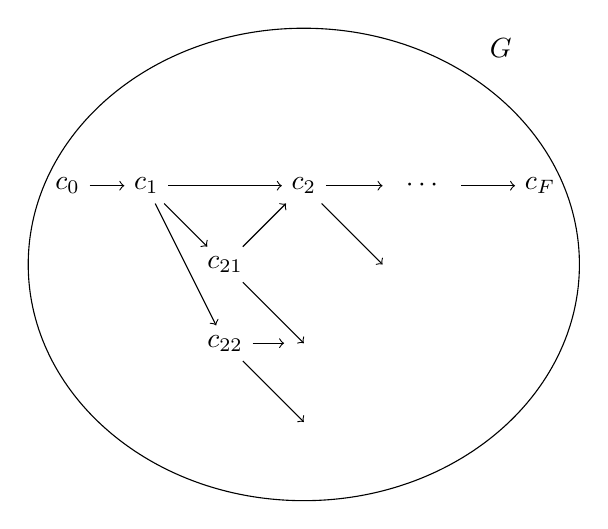
\begin{tikzpicture}
        \node (c0) at (0,0) {$c_{0}$};
        \node (c1) at (1,0) {$c_{1}$};
        \node (c2) at (3,0) {$c_{2}$};
        \node (c21) at (2,-1) {$c_{21}$};
        \node (c22) at (2,-2) {$c_{22}$};
        \node (cF) at (6,0) {$c_{F}$};
        \draw[->] (c0) -- (c1);
        \draw[->] (c1) -- (c2);
        \draw[->] (c1) -- (c21);
        \draw[->] (c1) -- (c22);
        \draw[->] (c21) -- (c2);
        \draw[->] (c21) -- +(1,-1);
        \draw[->] (c2) -- +(1,-1);
        \draw[->] (c2) -- +(1,0);
        \draw[->] (5,0) -- (cF);
        \draw[->] (c22) -- +(1,-1);
        \draw[->] (c22) -- +(0.75,0);
        \node () at (4.5,0) {$\cdots$};
        \draw (3,-1) ellipse [x radius=3.5cm, y radius=3cm];
        \node () at (5.5,1.75) {$G$};
    \end{tikzpicture}
\end{document}
